\documentclass[../main.tex]{subfiles}
\graphicspath{{\subfix{../img/}}}
\begin{document}

\newpage
\section{Simulator}

Der Simulator dient dazu, die Funktionalität der Software des autonomen Fahrzeugs zu testen, bevor der physische Prototyp gebaut wird.

\subsection{Spezifikation}

In diesem Abschnitt wird definiert, was der Simulator genau leisten soll.


% TODO: Transform to table 
\begin{itemize}
    \item Es wird (ohne Beachtung der Hindernisse) immer der schnellste Weg ins Ziel gefunden wird.
    \item Wegpunkte mit Pylonen werden nicht befahren.
    \item Entfernte Linien werden nicht befahren.
    \item Linien mit Hindernisse werden erkannt und nur befahren, falls ein Umweg länger dauert (konfigurierbar).
    \item Neue Informationen können während der Fahrt aufgenommen und entsprechende Anpassungen dazu getroffen werden.
    \item Kommandos, die an die Hardware geschickt werden sollen, werden aufgezeigt.
    \item Das Ziel kann konfiguriert werden (A, B oder C)
\end{itemize}



\subsection{Morphologischer Kasten}

% \begin{table}
%     \begin{tabularx}{l | a | b | a | b}
%     \hline
%     \rowcolor{LightCyan}
%     \mc{1}{}  & \mc{1}{x} & \mc{1}{y} & \mc{1}{w} & \mc{1}{z} \\
%     \hline
%     variable 1 & a & b & c & d \\
%     variable 2 & a & b & c & d \\ \hline
%     \end{tabular}
% \end{table}

\newcolumntype{Y}{>{\centering\arraybackslash}X}

\begin{table}[htbp]
    \centering
    \begin{tabularx}{\textwidth}{| X | Y | Y | Y |}
        \hline

        \rowcolor{LightGray}
        \textbf{Funktion} & \textbf{Option 1} & \textbf{Option 2} & \textbf{Option 3} \\ \hline
        
        \textbf{User Interface} &     
        Terminal \newline
        
\includegraphics[width=2.5cm]{img/simulation/morphologischer-kasten/terminal.png}
        &
        \cellcolor{LightGreen}
        Einfaches GUI \newline
        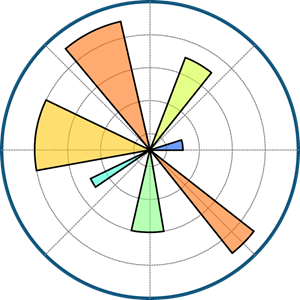
\includegraphics[width=2.5cm]{img/simulation/morphologischer-kasten/simple-gui.png}
        &
        Unreal Engine \newline
        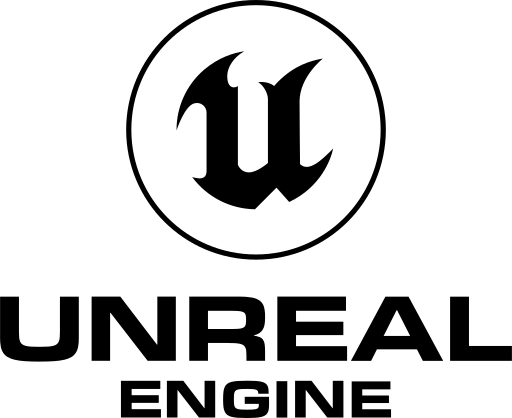
\includegraphics[width=2.5cm]{simulation/morphologischer-kasten/unreal-engine-logo.png}
        \\ \hline
        
        \textbf{Wegfindungs-Algorithmus}  &
        \cellcolor{LightGreen}
        Externe Bibliothek &
        Eigene Implementation &
        \\ \hline
        
        \textbf{Programmiersprache}      &
        \cellcolor{LightGreen}
        Python \newline
        
\includegraphics[width=2.5cm]{simulation/morphologischer-kasten/python.png} 
        &
        JavaScript \newline
        
\includegraphics[width=2.5cm]{simulation/morphologischer-kasten/javascript.png}
        &
        Java \newline
        
\includegraphics[width=2.5cm]{simulation/morphologischer-kasten/java.png}
        \\ \hline
        
        \textbf{Informationen \newline einlesen}  &     
        Bilder mit Objekterkennung \newline
        
\includegraphics[width=2.5cm]{img/simulation/morphologischer-kasten/ai-logo.jpg}
        &
        \cellcolor{LightGreen}
        Konfigurationsdatei \newline
        
\includegraphics[width=2.5cm]{simulation/morphologischer-kasten/yaml.png}
        &
        \\ \hline
        
        \textbf{Hindernis \newline Bewältigung}   &     
        Immer umfahren &
        Keine spezielle Behandlung &
        \cellcolor{LightGreen}
        Gewicht hinzufügen
        \\ \hline
    \end{tabularx}
\end{table}
\cellcolor{LightGreen}
\begin{itemize}
    \item User Interface
        \begin{itemize}
            \item Terminal
            \item \textbf{Einfaches GUI}
            \item Unreal Engine
        \end{itemize}
    \item Wegfindungs-Algorithmus
        \begin{itemize}
            \item \textbf{Externe Bibliothek}
            \item Eigene Implementation
        \end{itemize}
    \item Programmiersprache
        \begin{itemize}
            \item \textbf{Python}
            \item JavaScript
            \item Java
        \end{itemize}
    \item Informationen einlesen
        \begin{itemize}
            \item \textbf{Konfigurationsdatei}
            \item Bilder
        \end{itemize}
    \item Hindernis Bewältigung
        \begin{itemize}
            \item \textbf{Gewicht hinzufügen}
            \item Immer umfahren
            \item Keine spezielle Behandlung
        \end{itemize}
\end{itemize}

\subsubsection{User Interface}

Obwohl wir ebenfalls eine Unreal Engine mit dem Pfadfinder-Model erstellen, wäre der Aufwand zu gross, diesen an den Simulator anzubinden. Die Ausgabe in einem Terminal hingegen wäre zu minimal. Deshalb wird das User Interface mit einem einfachen GUI umgesetzt. 

\subsubsection{Wegfindungs-Algorithmus}

Der Wegfindungs-Algorithmus kann entweder selber oder mit Hilfe einer externen Bibliothek 
implementiert werden. Da für die Graphentheorie bereits viele beliebte Bibliotheken existieren, macht es für uns keinen Sinn, dies selbst zu implementieren. Zwar sind wir dadurch weniger flexibel, jedoch ist die Fehleranfälligkeit viel geringer.  

\subsubsection{Programmiersprache}

Bei der Programmiersprache kamen Python, JavaScript und Java in Frage.
Java wird für die meisten Projekte im Informatik-Studium verwendet. JavaScript erlaubt es, einfach graphische Darstellungen mittels Webseite zu implementieren. Python ist simpel und wird oft für Künstliche Intelligenz verwendet, was wir für die Implemetation der Software des autonomen Fahrzeugs benötigen. 

Wir entscheiden uns für Python, da viel know-how vorhanden ist. Ebenfalls bietet es mit NetworkX\footnote{https://networkx.org} eine mächtige Bibliothek für Graphen an.

\subsubsection{Informationen einlesen}

Damit die Software weiss, welche Hindernisse sich auf dem Graphen befindet, müssen Informationen eingelesen werden können. Idealerweise würde dies auf gleiche Art geschehen, wie in der Realität: anhand von Bildern mit Objekterkennung. Der Simulator soll jedoch so schnell wie möglich lauffähig sein, weshalb einfachkeitshalber eine Konfigurationsdatei mit den Informationen verwendet wird.

Dies könnte im späteren Verlauf von dem Projekt noch angepasst werden.

\subsubsection{Hindernis Bewältigung}

Der Simulator soll aufzeigen, wie mit Hindernissen umgegangen wird.
Hindernisse können eventuell nicht immer Umfahren werden, beispielsweise wenn alle anderen Pfade blockiert sind. Somit ist `Immer umfahren` keine gute Option. Hindernisse nicht speziell behandeln ist ebenfalls nicht optimal, da gleichlange Pfade ohne Hindernisse schneller durchfahren werden können. Deshalb verwenden wir die Option `Gewicht hinzufügen`. Dies erlaubt es uns, variabel zu entscheiden, wie viel Beachtung einem Hindernis geschenkt werden soll.

\subsection{Konzept}

Idealerweise würde der Simulator die komplette Hardware des autonomen Fahrzeuges simulieren. So wäre die Software, die auf dem Fahrzeug läuft, genau die gleiche, die vom Simulator getestet wird. Dies ist jedoch mit sehr viel Aufwand verbunden, weshalb dies für die erste Version des Simulators für uns nicht realisierbar ist.

Die erste Version des Simulators soll anhand einer vordefinierten Konfiguration den schnellsten Weg ins Ziel finden. Die Konfiguration enthält folgende Informationen:
\begin{itemize}
    \item Das Ziel: A, B oder C.
    \item Die Gewichtung für das Befahren eines Hindernis.
    \item Informationen die erst beim Befahren eines neuen Wegpunktes freigeschalten werden:
     \begin{itemize}
        \item{Wegpunkte mit einem Pylon}
        \item{Entfernte Linien}
        \item{Erkannte Hindernisse}
   \end{itemize}
\end{itemize}


Damit die Simulation weiss, auf welchen Wegpunkten bzw. Linien sich Hindernisse befinden, wird jeder Wegpunkt beschriftet:

\imagewidth{simulation/labeled-graph.png}{Beschrifteter Graph}{10cm}

Die Konfiguration wird in einer YAML-Datei abgespeichert und sieht wie folgt aus.

\begin{verbatim}
end: B
weight: 3
S:
  cones: [E]
  obstacles: 
    - [S, F] 
  removed:
    - [E, A]
D:
  removed:
    - [D, B]
  obstacles:
    - [D, A]
\end{verbatim}

In der Beispielskonfiguration wird das Ziel B angesteuert.
Eine Line mit Hindernis wird dreifach gewichtet im Vergleich zu einer normaler Line.  
Am Start (Knote S) erfährt die Software, dass auf dem Knoten E sich eine Pylone befindet,
auf der Linie S-F ein Hindernis und dass die Linie E-A entfernt wurde.
Falls das Fahrzeug die Kante D befährt, wird erkannt, dass die Kante D-B nicht existiert und dass sich auf Kante D-A ein Hindernis befindet.

Diese Konfiguration kann einfach angepasst werden, wodurch mit dem Simulator einfach verschiedene Szenarien durchgespielt werden können.


\subsubsection{Nutzwertanalyse}
\textbf{TODO: Benötigt anpassungen}
Die Wegfindung und Entscheidungsprozesse des Fahrzeugs sollen anhand eines Simulators und vor dessen Bau getestet werden können. Bei der Technologierecherche wurden zwei Methoden recherchiert, die in diesem Abschnitt genauer analysiert werden.
Der passendste Simulator wird anhand einer Nutzwertanalyse mit den folgenden Kriterien gewählt.

\begin{itemize}
\item \textbf{Anpassbarkeit}: Das wichtigste Kriterium ist, dass der Simulator genau an die Problemstellung angepasst werden kann.
\item \textbf{Geschwindigkeit}: Die Simulation soll auf handelsüblichen Rechnern mit moderater Leistung schnell laufen, um einfache Softwareiteration zu ermöglichen.  
\item \textbf{Komplexität}: Das Projekt ist zeitlich limitiert. Der Aufwand für die Implementierung und Anpassung des Simulators muss berücksichtigt werden.
\item \textbf{Schnittstellen}: Damit der Simulator angesteuert werden kann, soll er möglichst einfache Schnittstellen besitzen.
\end{itemize}


\begin{table}[H]
\resizebox{\textwidth}{!}{

 \centering
 \renewcommand{\arraystretch}{1.5}
     \begin{tabular}{|c|c|c|c|c|c|c|c|c|c|}
        \hline
        \multicolumn{2}{|c|}{} & 
        \multicolumn{2}{c|}{\textbf{Selbst entwickelt}} &
        \multicolumn{2}{c|}{\textbf{MicroMouseSimulator}}\\ 
        \hline
        
        \textbf{Kriterium} & \textbf{Gewicht} &
        \textbf{Bewertung} & \textbf{Punkte} &
        \textbf{Bewertung} & \textbf{Punkte}\\
        \hline

        Anpassbarkeit & 40 &
        10 & 360 &
        5 & 200 \\
        \hline

        Schnittstellen & 30 &
        10 & 300 &
        8 & 240  \\
        \hline

        Komplexität & 20 &
        8 & 160 &
        4 & 80 \\
        \hline

        Geschwindigkeit & 10 &
        8 & 80 &
        9 & 90 \\
        \hline


        
        \textbf{Nutzwert:} & 100 & & 900 & & 610\\ \hline
    \end{tabular}
 }
    \caption{Nutzwertanalyse Simulator}
    \label{tab:nutzwertanalyse_simulator}
\end{table}

Ein selbstgebauter Simulator erreicht in der durchgeführten Nutzwertanalyse (siehe Tabelle \ref{tab:nutzwertanalyse_simulator}) die beste Gesamtbewertung. Das hohe Mass an Anpassbarkeit und die Möglichkeit, Schnittstellen nach Belieben zu implementieren, sprechen klar für eine Eigenentwicklung. Der MicroMouseSimulator ist bereits auf Geschwindigkeit optimiert, jedoch sollte der Unterschied auf modernen Rechnern einen zu kleinen Unterschied machen, als dass die anderen Nachteile aufgeholt würden. Statt sich in den Source-Code eines bereits bestehenden Projektes einzulesen, kann von Grund auf für die vorhandene Problemstellung entwickelt werden.

\end{document}